\section{Pengenalan UI (User Interface) dan UX (User Experience)}

Dalam pengembangan web, dua istilah yang sangat sering digunakan adalah \textbf{UI} (User Interface) dan \textbf{UX} (User Experience). Meskipun keduanya saling berkaitan erat, keduanya merujuk pada aspek yang berbeda dari produk digital. Pemahaman yang tepat tentang perbedaan dan hubungan keduanya sangat penting bagi pengembang web, karena produk yang sukses memerlukan keunggulan di kedua aspek ini \cite{mdnLearn}.

\textbf{User Interface (UI)} adalah segala sesuatu yang \textit{terlihat dan dapat diinteraksi} oleh pengguna: tombol, menu, formulir, ikon, tipografi, warna, dan tata letak. UI adalah ``wajah'' dari produk---kesan pertama yang diterima pengguna saat membuka aplikasi web. Desain UI yang baik bersifat konsisten, estetis, dan intuitif secara visual. UI yang buruk---misalnya tombol yang terlalu kecil, warna kontras rendah, atau tata letak yang berantakan---membuat pengguna frustrasi meskipun fungsionalitas sistemnya lengkap \cite{webdevLearn}.

\textbf{User Experience (UX)} adalah keseluruhan pengalaman pengguna saat berinteraksi dengan produk, mulai dari perasaan pertama kali melihat halaman hingga keberhasilan menyelesaikan tugas. UX mencakup aspek yang lebih luas daripada UI: kemudahan penggunaan (\textit{usability}), kecepatan, aksesibilitas, alur navigasi, dan bahkan emosi pengguna. Seseorang mungkin melihat antarmuka yang cantik (UI bagus), tetapi jika tidak bisa menyelesaikan tugasnya karena alur yang membingungkan, maka UX-nya buruk \cite{nngroup}.

\begin{table}[htbp]
\centering
\begin{tabular}{|P{3cm}|P{4.5cm}|P{4.5cm}|}
\hline
\textbf{Aspek} & \textbf{UI (User Interface)} & \textbf{UX (User Experience)} \\
\hline
Fokus & Tampilan visual dan interaksi & Keseluruhan pengalaman pengguna \\
\hline
Pertanyaan kunci & ``Apakah tampilannya menarik dan jelas?'' & ``Apakah pengguna dapat menyelesaikan tugasnya?'' \\
\hline
Elemen & Warna, tipografi, ikon, layout, tombol & Alur, kecepatan, emosi, kepuasan \\
\hline
Analogi & Tampilan dashboard mobil & Pengalaman berkendara keseluruhan \\
\hline
Keahlian & Desain grafis, visual design & Riset pengguna, information architecture \\
\hline
\end{tabular}
\caption{Perbandingan UI dan UX}
\end{table}

\subsection{Hubungan UI dan UX}

UI dan UX bukanlah dua hal yang terpisah sepenuhnya, melainkan saling melengkapi. Analogi yang tepat: UI adalah \textbf{pelana kuda}---tampilan, bahan, dan detail jahitan---sedangkan UX adalah \textbf{pengalaman menunggang}---kenyamanan, kontrol, dan kepuasan berkuda. Pelana yang indah tetapi tidak nyaman diduduki adalah UI bagus tetapi UX buruk. Pelana yang nyaman tetapi jelek dipandang adalah UX bagus tetapi UI kurang menarik. Produk terbaik menyeimbangkan keduanya \cite{webdevLearn}.

\begin{figure}[htbp]
\centering
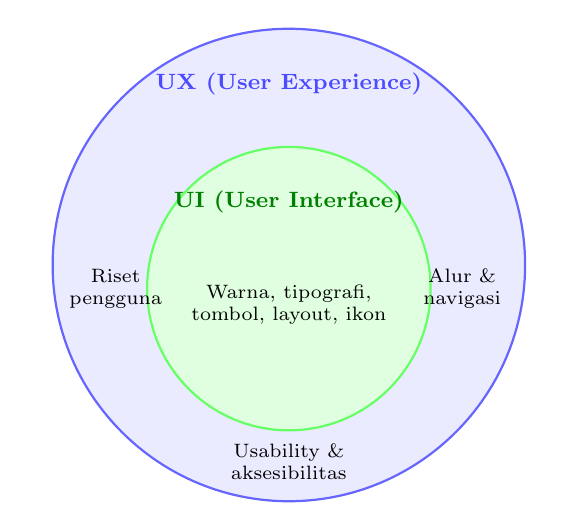
\begin{tikzpicture}[transform shape, every node/.style={font=\footnotesize}]
  % UX circle (larger)
  \draw[fill=blue!8, draw=blue!60, thick] (0,0) circle (3cm);
  \node[font=\footnotesize\bfseries, blue!70] at (0, 2.3) {UX (User Experience)};
  
  % UI circle (smaller, inside UX)
  \draw[fill=green!12, draw=green!60, thick] (0,-0.3) circle (1.8cm);
  \node[font=\footnotesize\bfseries, green!50!black] at (0, 0.8) {UI (User Interface)};
  
  % Labels inside
  \node[text width=2.8cm, align=center, font=\scriptsize] at (0, -0.5) {Warna, tipografi,\\ tombol, layout, ikon};
  
  % Labels in UX ring
  \node[font=\scriptsize, text width=2cm, align=center] at (-2.2, -0.3) {Riset\\pengguna};
  \node[font=\scriptsize, text width=2cm, align=center] at (2.2, -0.3) {Alur \&\\navigasi};
  \node[font=\scriptsize, text width=2cm, align=center] at (0, -2.5) {Usability \& aksesibilitas};
\end{tikzpicture}
\caption{Hubungan UI dan UX: UI adalah bagian dari UX yang lebih luas}
\end{figure}

\subsection{Prinsip Dasar UI/UX untuk Web}

Beberapa prinsip dasar yang harus dipahami oleh setiap pengembang web antara lain: (1) \textbf{Konsistensi}---elemen yang sama harus berperilaku dan tampil sama di seluruh halaman; (2) \textbf{Umpan balik} (\textit{feedback})---sistem harus memberikan respons yang jelas atas setiap tindakan pengguna (misalnya, tombol berubah warna saat diklik); (3) \textbf{Hierarki visual}---elemen terpenting harus paling menonjol; (4) \textbf{Kesederhanaan}---jangan membebani pengguna dengan terlalu banyak pilihan di satu layar; dan (5) \textbf{Aksesibilitas}---desain harus dapat digunakan oleh semua orang, termasuk pengguna dengan disabilitas \cite{mdnAccessibility}.

\begin{konsep}
\textbf{UI tanpa UX = Bungkus cantik tanpa isi.} Pengguna mungkin terkesan saat pertama kali melihat, tetapi akan frustrasi saat tidak bisa menyelesaikan tugasnya. \textbf{UX tanpa UI = Isi bagus, bungkus jelek.} Pengguna mungkin bisa menyelesaikan tugas tetapi tidak menikmati prosesnya dan enggan kembali. Produk web terbaik menggabungkan keduanya: antarmuka yang indah \textit{dan} pengalaman yang mulus.
\end{konsep}
